\chapter{Continuous Static Analysis Tool Design}
\label{ch:kiskadee}

In Free/Libre and Open Source Software (FLOSS) projects, a
common source of bug reports are the GNU/Linux distributions.
These distributions ship thousands of software projects, which
they call packages. Distribution developers refer to the
projects that maintain the software they ship in the
distribution as \textit{upstream}.  It is not unusual for
distribution developers to report bugs in upstream projects or
to send patches to fix bugs found by their distribution users
or during the packaging process. Figure
\ref{fig:floss_bugs_workflow} shows a typical bug reporting
workflow, where users report the bugs they find to the
distribution developers, who in turn report these bugs (in
addition to bugs found during the packaging process) to the
upstream project maintainers of the package containing the bugs.

\begin{figure}[!h]
  \centering
  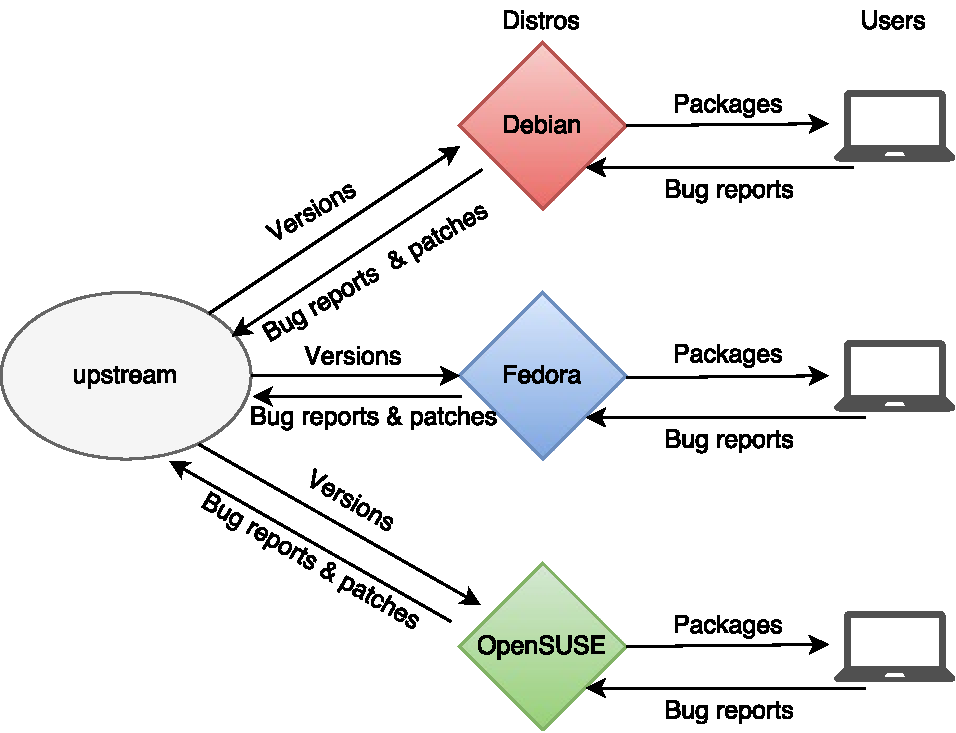
\includegraphics[width=.75\textwidth]{figures/floss_bugs_workflow} 
  \caption{FLOSS bug report workflow.}
  \label{fig:floss_bugs_workflow} 
\end{figure}

By continuously running multiple static analyzers in several of these packages,
i.e., once for each version of the package, we can create a database of static
analysis reports on software projects of different sizes and application
domains. Developers can then use the information in this database to find and
act on software flaws.

We chose to use GNU/Linux distributions due to the high amount
of software packages available and the well-defined and
documented interfaces they provide to download the latest
versions of these packages. It is also an advantage that the
cultural norm for GNU/Linux distribution developers is to
report (and often propose fixes for) bugs. Therefore, using
their repositories for this work may provide a broader user
base for the tools and techniques developed in this research.

\section{Features and System Overview}
\label{sec:system_overview}

\begin{figure}[hbt]
\centering
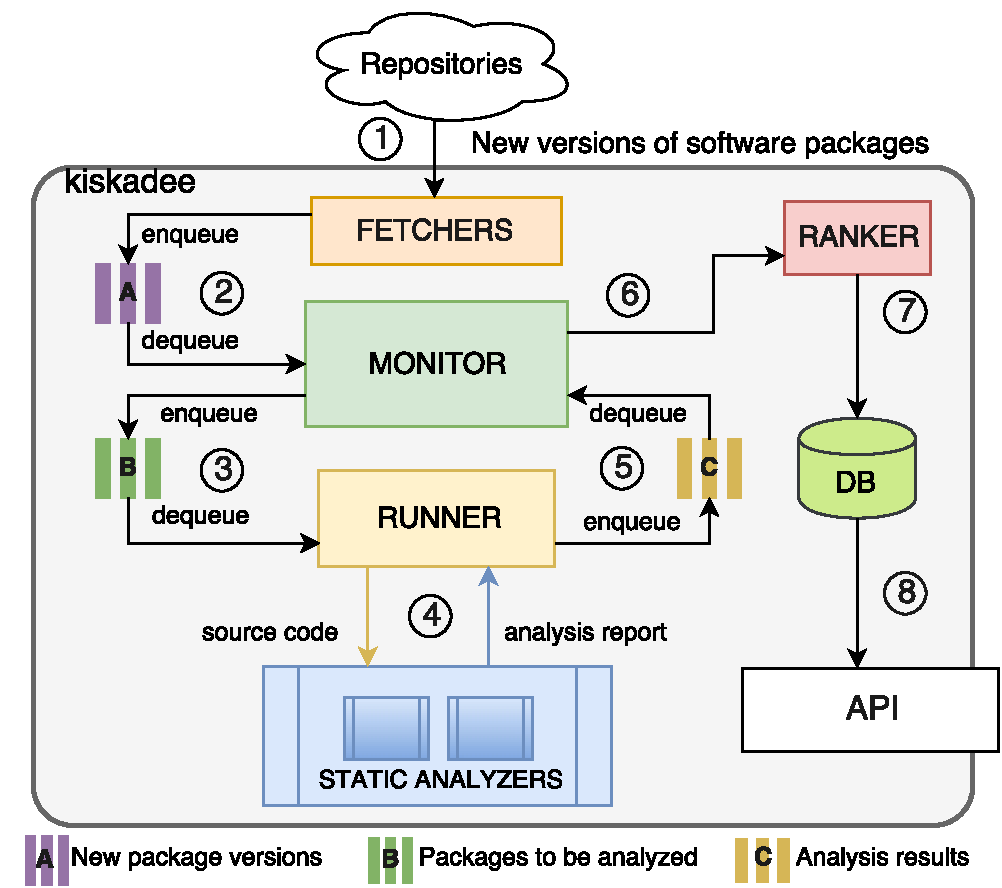
\includegraphics[width=.75\textwidth]{figures/kiskadee-overview.pdf}
  \caption{kiskadee design overview.}\label{fig:kiskadee:overview}
\end{figure}

To continuously run static analysis on software packages and handle the false
alarms generated by these analyses, we developed \textit{kiskadee}. Its main features are described below:

\begin{enumerate}
\item \textbf{Monitor specific software repositories for new releases.} This way, we can track and analyze each release of the monitored packages since we started monitoring them.

\item \textbf{Download new software packages from the repositories.}

\item \textbf{Run multiple static analyzers on the downloaded packages.}

\item \textbf{Translate each static analyzer report to a common report format.} This is needed to enable analyzing the reports during the ranking and visualization phase. Since the system is extensible, we do not want to write parsing rules for each static analyzer report format to compare the analyzers, so we do this before saving the static analysis output.

\item \textbf{Rank warnings.} The warnings are ranked based on their probabilities of being true of false positives. The methodology and techniques applied to implement this feature are described in Chapter~\ref{ch:ranking}.

\item \textbf{Save the reports in a database.}

\item \textbf{Make data available through an API.}

\item \textbf{Present data to users on a web user interface.} Users can filter warnings per package name and version.
\end{enumerate}

Figure~\ref{fig:kiskadee:overview} represents kiskadee's architecture overview,
where the numbers denote its execution flow.
\begin{itemize}
  \item In steps (1) and (2), kiskadee
monitors software repositories for new releases.
    \item In step (3), kiskadee
downloads the source code of each new software version in a repository it
monitors and runs a set of predefined static analyzers on it in step (4).
    \item In step (5),
kiskadee translates each static analyzer report to a common warnings report format.
This common format is needed because each static analyzer defines
its unique format to report warnings.
    \item In step (6), kiskadee ranks the warnings
based on their probability of being real bugs, where warnings on the top have a
higher probability of being real bugs and warnings on the bottom are more
likely to be false positives. To perform this ranking step, we use a
classification model, described in Chapter~\ref{ch:ranking}.
    \item The ranked
warnings are then saved in a database in step (7), using kiskadee's common
warning report format.  
    \item Finally, in step (8), kiskadee provides an API consumed
by a visualization tool to display the ranked warnings filtered by package
versions. The information provided can be used either by distribution developers to
evaluate and report possible bugs upstream or by upstream developers
themselves. Researchers can also use kiskadee's database in different contexts.
\end{itemize}

The next sections describe important details related to
kiskadee features. Then, in Section~\ref{sec:implementation}, we discuss
kiskadee's architecture and implementation details. We finish the chapter by discussing software projects related to kiskadee in Section~\ref{sec:related_projects}.

\section{Monitoring Software Repositories}
\label{sec:monitoring}

Although pointing kiskadee to GNU/Linux distribution repositories may have
advantages, most distributions do not package every single new software version
for the packages it distributes. Different reasons lead to the non inclusion of
some software versions in distributions. For instance, some software projects
claim that they only provide stable software every other release.  Other
projects release versions too fast, making the effort of packaging every single
release pointless to the distribution packager.

Fedora Project uses an external system to monitor the software projects they
distribute. Anitya~\cite{anitya} maps upstream projects to distribution package
names. Whenever a new version of an upstream project is released, Anitya
publishes the new release in a Fedora infrastructure publish-subscribe system
where other systems in the distribution infrastructure can handle it. New
software versions are published by Anitya as soon as they are released
upstream. Analyzing these new software versions with kiskadee as early as they
are released allows the distribution developers to address potential bugs found
by kiskadee before the software is shipped to final users. It also ensures that
every new monitored software release gets analyzed, even if the new version is not
packaged in the distribution, for the reasons aforementioned. Therefore,
kiskadee monitors packages by reading information published by Anitya in the
Fedora infrastructure publish-subscribe system.

kiskadee can monitor other software repositories as well through its plugin
architecture (kiskadee's fetchers). Each fetcher must implement functions that
define which repository to monitor, how to monitor it, and which static
analyzers to run for that repository. Hence, we can extend \textit{kiskadee} to
run different static analyzers for different software repositories or GNU/Linux
distributions.

\section{Static Analyzers}
\label{sec:analyzers}

The NIST Software Assurance Metrics and Tool Evaluation (SAMATE) project
provides a list of \textit{source code security
analyzers}\footnote{\url{samate.nist.gov/index.php/Source_Code_Security_Analyzers.html}},
which they define as static analyzers that \textit{examine source code to
detect and report weaknesses that can lead to security vulnerabilities}.

We ran\textit{kiskadee} with three static analysis tools to generate the
warnings data set for our experiments. Based on SAMATE tools list and
references, the criteria to select the tools were:
\begin{enumerate}
  \item \textbf{The tools must be able to examine C/C++ code for security flaws (e.g., buffer overflows, null pointer dereferences).} Different programming languages have different problems, and we do not want to address this variable at the moment. Since C and C++ programming languages are often used to develop critical software systems and several software flaws are mapped under Common Weakness Enumeration (CWE) for these languages, we chose to work with these languages.
  \item the tool source code must be released under a FLOSS license.
\end{enumerate}
Criterion~1 ensures the tool can analyze a subset of the test cases in our data
set, introduced in Section~\ref{sec:data}, whereas criterion 2 preserves us
from disputes by tool vendors regarding the analysis of the results (such as
allegations of sub-optimal tool calibration or detrimental calculation
methodology)\footnote{In fact, if we chose
to work with
proprietary tools, we would need to contact the vendors about our experiments
and request permission before publishing our results.}. FLOSS tools also simplify the process of retrieving string
constructs for static analyzer warning messages and categories when necessary,
since we can verify their source code.

Following the criteria, the static
analyzers selected were \emph{Clang Static Analyzer} (version 3.9.1),
\emph{Cppcheck} (version 1.79), and \emph{Frama-C} (version 1.14 with the value
analysis plugin activated).

\textit{Frama-C} with its value analysis plug-in was the first choice since it
was the tool used for the Ockham Criteria~\cite{black_sate_2016} and the
authors claim Frama-C is a sound tool, not producing false positives, which may
help on the ranking phase of this study. It uses abstract interpretation
techniques. Although SAMATE does not list Frama-C in its recommended tools list, it
is recommended by the Flawfinder
website\footnote{\url{dwheeler.com/flawfinder}}, one of the secondary tool
lists recommended by SAMATE. Next \textit{Cppcheck} was chosen, which is a
static analyzer that works by matching on tokens, without more in-depth analysis
methods. Cppcheck authors also claim to avoid generating false positives.
Finally, \textit{Clang Static Analyzer} works by performing inter-procedural
analysis on the source code and, differently from the other two selected tools,
the authors do not claim that this tool does not generate false positives.

Table~\ref{tab:selected_tools} shows the tools integrated into kiskadee. The same tools were also employed to generate
our experimental data set, as we discuss in Chapter~\ref{ch:ranking}.

  \begin{table}
    \centering
    \begin{threeparttable}
    \begin{center}
        \begin{tabular}{rcrc}\hline
          Tool & Target Language & License & Version \\
        \hline
          Clang Static Analyzer & C/C++ & NCSA/MIT & 3.9.1\\
          Cppcheck & C/C++ & GPLv3 & 1.79\\
          Frama-C$^{*}$ & C & LGPLv2 & 1.14 \\ \hline
        \end{tabular}
        \begin{tablenotes}
          \small
        \item[*] \footnotesize{Although Frama-C cannot analyze C++ code, it meets criterion~1 by analyzing a substantial subset of Juliet test cases. Frama-C was used with its value analysis plugin activated.}
        \end{tablenotes}
        \caption{Selected static analysis tools}\label{tab:selected_tools}
    \end{center}
    \end{threeparttable}
\end{table}

We designed kiskadee in an extensible fashion. Whenever the desire to
integrate new static analyzers to it arises, the effort needed to do so is
decoupled from kiskadee source code. Instead, one would just need to extend the
external common reporting language library used by kiskadee to parse and
convert the target static analyzer report to the common report. We now, we
discuss this common reporting language.

\section{Common Reporting Language}
\label{sec:firehose}

A previous work has discussed the problem of having a common reporting language
for static analyzers. By applying the Ockham Sound Analysis
Criteria~\cite{black_sate_2016}, we designed a simplified common bug report
format to compare known bugs with bug reports from the tools evaluated with the
criteria. The criteria data and programs to reproduce results are available in
the SATE V Ockham Sound Analysis Criteria NIST Internal Report
\cite{black_sate_2016}, where the bug report formats specified can be retrieved
from and replicated. While the format was fit to perform the analysis, we
designed it on top of the criteria concepts and the tools used for the criteria,
which needed the following information:

\begin{itemize}
\item a specific location for the bug;
\item the type of the bug being reported (related to a CWE);
\item a code snippet with the buggy code;
\item information to identify false alarms on that code snippet.
\end{itemize}

We defined an XML format to extract information from the used test suite (code
snippets with known flaws injected) to verify the soundness of the analyzed
tools. Listing~\ref{lst:ockham_xml} is an example of the format, extracted from
one of the files with Ockham results.  Although tools to extract information
from the format were developed and are available, no formal definition of the
format was described, since this format was used for this specific version of
the criteria.

\begin{minipage}{\linewidth}
\begin{lstlisting}[frame=none, caption={Ockham Criteria XML bug report example},label={lst:ockham_xml}]
<?xml version='1.0' encoding='utf-8'?>
<sites>
  <file name="CWE369_Divide_by_Zero__int_fgets_divide_51b.c">
    <site type="div_by_zero" line="27" info="data" val="buggy">
      <code><![CDATA[printIntLine(100 / data);]]></code>
    </site>
    <site type="div_by_zero" line="38" info="data" val="good">
      <code><![CDATA[printIntLine(100 / data);]]></code>
    </site>
    <site type="div_by_zero" line="47" info="data" val="good">
      <code><![CDATA[printIntLine(100 / data);]]></code>
    </site>
  </file>
</sites>
\end{lstlisting}
\end{minipage}

To compare the findings of the evaluated tools with actual data from the test suite, we parsed
the tool reports and converted them to a straightforward comma-separated values
(CSV) format containing \textit{file name}, \textit{line} and \textit{bug category
related to a CWE}. An example of this CSV format, extracted from the Ockham
Criteria results, is shown in Listing~\ref{lst:ockham_csv}.

\begin{minipage}{\linewidth}
\lstset{language=Python}
\begin{lstlisting}[frame=none, caption={Ockham Criteria CSV bug report example},label={lst:ockham_csv}]
CWE121__char_type_overrun_memcpy_01.c, 43, divByZero
CWE121__char_type_overrun_memcpy_01.c, 62, divByZero
CWE121__char_type_overrun_memcpy_02.c, 45, divByZero
CWE121__char_type_overrun_memcpy_02.c, 73, divByZero
CWE121__char_type_overrun_memcpy_02.c, 92, divByZero
CWE121__char_type_overrun_memcpy_03.c, 45, divByZero
CWE121__char_type_overrun_memcpy_03.c, 73, divByZero
CWE121__char_type_overrun_memcpy_03.c, 92, divByZero
CWE121__char_type_overrun_memcpy_04.c, 51, divByZero
CWE121__char_type_overrun_memcpy_04.c, 79, divByZero
\end{lstlisting}
\end{minipage}

To rank warnings, we would like to have information on analyzed software
versions, which static analyzer performed the analysis, the version of the
analyzer, the severity of the problem found, and the string message given by the
analyzer. All this information may be interesting for research or bug reporting
purposes. Thus, if we were to use the format we developed for the Ockham Criteria,
changes would be needed, both to the format and to the tools provided to work
with it.

FLOSS development communities have also been discussing a common static
analysis report output format. The Fedora Project Static Analysis Special
Interest Group (SIG)~\cite{fedora:static:sig} designed a tool to run static analyzers
during the
package build process \cite{fedora:mockwithanalysis}.  Although the tool itself
is in its early development stages and not ready for usage in production, the
developers discussed a common report format for the static
analyzers in their mailing lists~\cite{fedora:mlist}. After a few iterations, with Debian Project
developers collaboration, they created and evolved \textit{Firehose}, a complete definition
of a common warnings report format for static analyzers and a set of tools to
generate, parse, and verify this format.
\textit{Firehose} addresses the issues previously discussed, as analyzer name
and version, optional fields for severity, and complete warning messages. It also allows custom fields in the format, which we use to include kiskadee's ranking information.
Appendix \ref{apx:firehose} is a RELAX-NG schema describing the
\textit{firehose} format.
We use \textit{Firehose} as kiskadee's
common warning report format, eliminating the need to design a new format and
to develop the tools to handle it, like parsers and generators.

Moreover, as previously  mentioned in Section~\ref{sec:analyzers}, if we want
to integrate new static analyzers to kiskadee, this must be performed in
Firehose, by implementing a new parser for the target static analyzer. During
the Google Summer of Code
2017\footnote{\url{https://summerofcode.withgoogle.com/}} program, we extended
Firehose to parse both the Frama-C static analyzer, which we use for our
experiments described in Chapter~\ref{ch:ranking}, and the Flawfinder static
analyzer.

\section{API and Web User Interface}
\label{sec:api}

To provide the static analysis reports and warnings ranking data to external
applications, kiskadee exposes an API. The API responses contain the following information:

\begin{itemize}
  \item List of all active fetchers running in kiskadee's current instance.

  \item List of all packages analyzed by kiskadee up to the time of the API request.

  \item List of each version analyzed for a given package.

  \item The full analysis report for each package version analyzed, in the Firehose format. Also includes ranking information.
\end{itemize}

Provided with this API and aided by students at University of Brasília (UnB),
we developed a user interface (UI) for kiskadee. We based many of the UI ideas
on concepts previously discussed by the Fedora Static Analysis SIG on the
project development mailing lists. Proper credits and acknowledgements for the
UnB contributions can be found in the \emph{Acknowledgements} section in the
beginning of this document.

Figure~\ref{fig:kiskadee-main}, Figure~\ref{fig:kiskadee-list}, and
Figure~\ref{fig:kiskadee-list-complete} show some screens of the UI developed
by the students. The next section presents more speific details on kiskadee's
implementation.

\begin{figure}[!h]
  \centering
  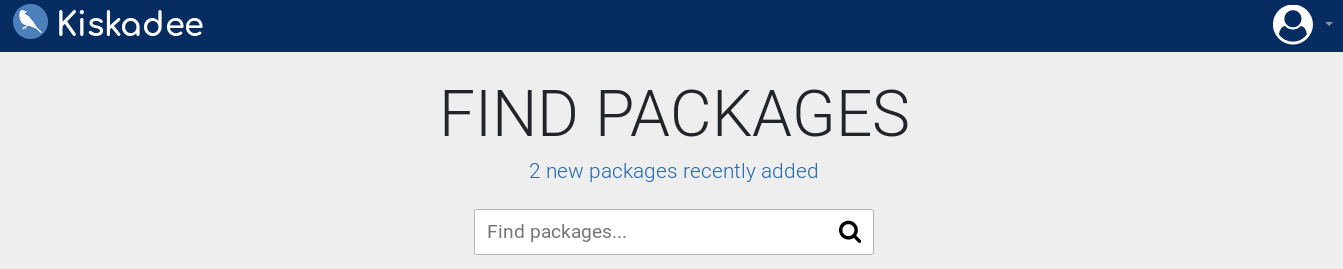
\includegraphics[width=.95\textwidth]{figures/kiskadee-main} 
  \caption{kiskadee UI: Package search page}
  \label{fig:kiskadee-main} 
\end{figure}

\begin{figure}[!h]
  \centering
  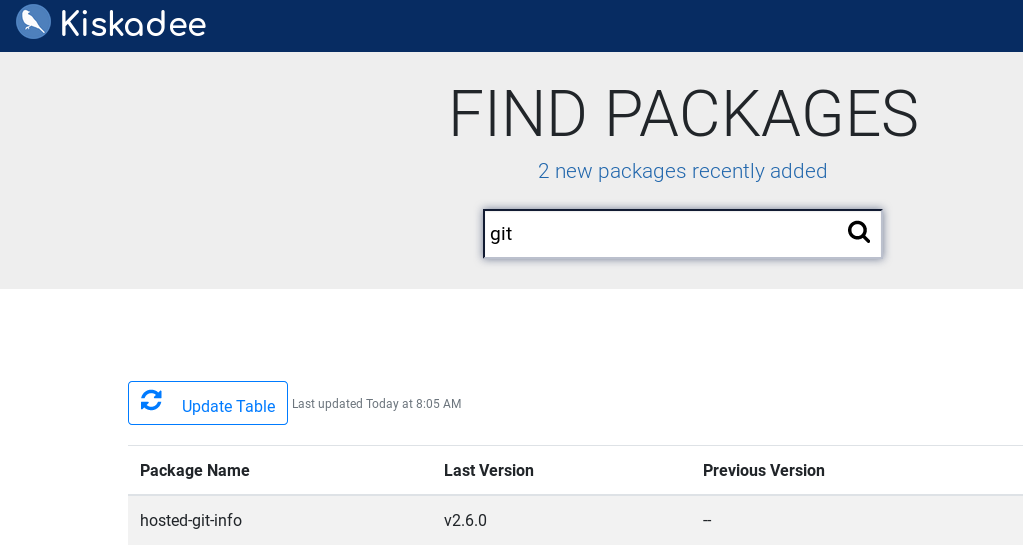
\includegraphics[width=.95\textwidth]{figures/kiskadee-list} 
  \caption{Kiskadee UI: List and versions of analyzed packages}
  \label{fig:kiskadee-list} 
\end{figure}

\begin{figure}[!h]
  \centering
  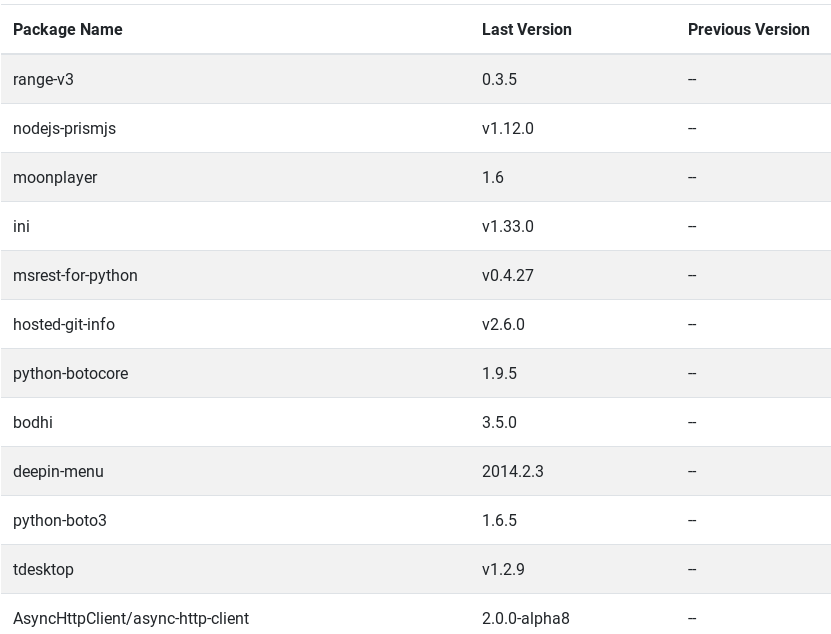
\includegraphics[width=.95\textwidth]{figures/kiskadee-list-complete} 
  \caption{Kiskadee UI: Comprehensive list of analyzed packages}
  \label{fig:kiskadee-list} 
\end{figure}

\section{Architecture and Implementation Details}
\label{sec:implementation}

kiskadee's architecture aims to decouple source code analysis from software
packages release monitoring. To accomplish that, we have separated the modules
responsible for fetching package versions and source code, and the module
responsible for running the analyses. The communication between them is done through
queues, as shown in Figure~\ref{fig:kiskadee:overview} by \textbf{A},
\textbf{B}, and \textbf{C}.

The packages\_queue (\textbf{A}) is used by the fetchers to enqueue the
packages that should be analyzed. The monitor module consumes this queue
to check if the enqueued package was already analyzed. The second queue, named
analysis\_queue (\textbf{B}), is consumed by the runner module to receive
packages that must be analyzed, which are enqueued by the monitor module. If a
dequeued package does not have an analysis instance in the database, the
monitor module enqueues it for analysis in the analysis\_queue.  When an
analysis is performed, the runner module sends the analysis report to the
monitor module, by enqueuing it in the results\_queue (\textbf{C}). Some package
metadata and the analysis are then saved in the database by the monitor module.

The \emph{fetchers} module implements a system to easily define targets to be
monitored by kiskadee. A target is a software repository monitored for new
packages. Whenever kiskadee is loaded, it loads all fetchers installed in a
specific path. From that moment on, kiskadee starts monitoring all the targets
defined by the loaded fetchers.

A new fetcher must inherit from kiskadee's Fetcher and implement some required
abstract methods so kiskadee knows how to

\begin{itemize}
  \item monitor the target;
  \item download source code; and
  \item compare target's software versions.
\end{itemize}

Listing~\ref{lst:fetcher} shows a complete example of a custom kiskadee fetcher implementation.

\begin{minipage}{\linewidth}
\lstinputlisting[frame=none, caption=Example kiskadee fetcher, style=mypython, label={lst:fetcher}]{listings/example.py}
\end{minipage}

A few different software projects overlap with certain kiskadee features. We
finish this chapter by listing and discussing some of these software projects
in the next section.

\section{Related Projects}
\label{sec:related_projects}

\subsection{Debile}

Debian Project has been developing Debile, a reduced Debian build system to aid
developers to build packages or run custom tools against source or binary
packages.  Debile can run multiple static analyzers in Debian repository
packages and return the reports in the \textit{firehose}
format (\url{https://github.com/opencollab/debile}). While the tool is
still in early development (not in production), kiskadee design was inspired in
Debile, with some simplifications and abstractions, allowing us to fetch source
code from different software repositories. While Debile aims to check the
quality of Debian packages, kiskadee focus on a broader scope, being
distribution agnostic and fetching software packages from the upstream projects.

\subsection{mock-with-analysis}

Similar to Debile, mock-with-analysis
(\url{https://github.com/fedora-static-analysis/mock-with-analysis}) is a
command line tool to build RPM\footnote{\url{rpm.org}} packages in a clean
chroot and run multiple static analyzers on the source code of the package
being built. This tool is based on
mock~\footnote{\url{https://github.com/rpm-software-management/mock}}, a tool
used by Fedora developers to build RPM packages in a clean environment with a
minimum set of packages pre-installed. While mock-with-analysis is just a
prototype at the moment and is not fit for general usage, it inspired the
development of Firehose, which is an essential component for kiskadee.

\subsection{Coala}

Coala (\url{https://coala.io}) provides a single interface to run multiple
static analyzers in software packages written in numerous programming languages
and producing a report in a common reporting language defined by the Coala
project. The tool is not restrained to security oriented static analysis, it
also runs linters and other analyzers to check code quality and style.

While all the projects mentioned above are interesting projects, and Coala
being a production-level open source software sponsored by large companies,
none of them proposes an approach to reduce the number of false positive
warnings generated by the analysis, which increases when running multiple
static analyzers in a software package. In the following chapter, we present
our approach to handling these false positives by training a classification model
and ranking the warnings based on classification probabilities.

